\subsection{Общая схема электронного документооборота} \label{doc_scheme}

% \textbf{\textit{Документооборот}} -- движение документов в организации с момента их создания или получения до завершения исполнения или отправления.\cite{bib1}


\begin{figure} [h] 
  \center
  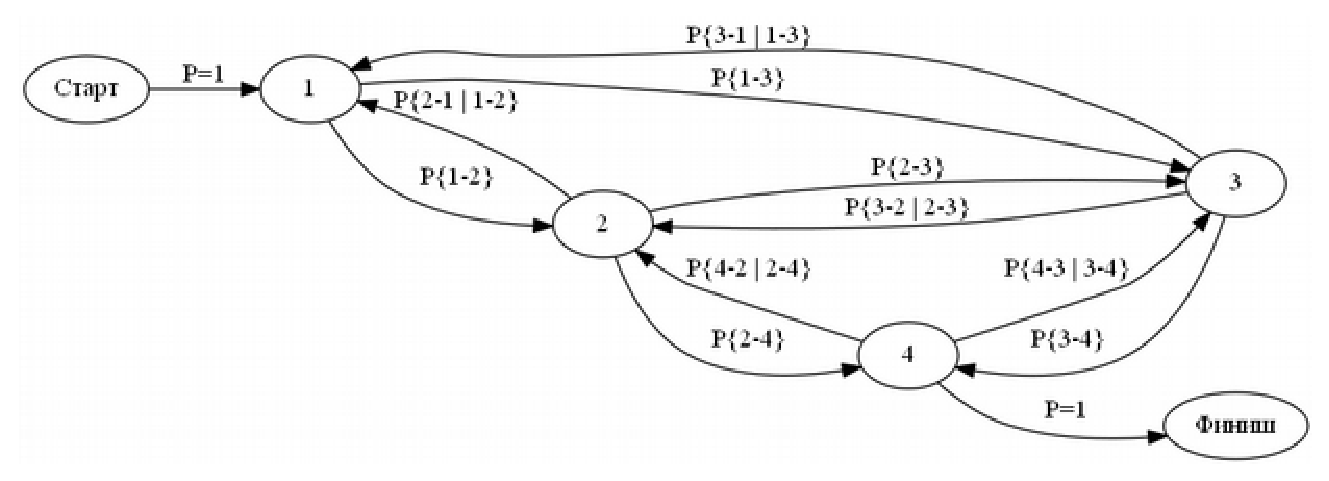
\includegraphics [scale=0.7] {graph1}
  \caption{Характерный вид процесса документооборота} 
  \label{img:graph1}  
\end{figure}

Процесс документооборота можно представить в виде графа, изображённого на рис. \ref{img:graph1}. Вершинами в нём являются редакторы, а дугами -- переходы задания на разработку документа между редакторами в соответствии с принятой в организации структурой. Весам дуг соответствуют вероятности этих переходов. Обратные связи демонстрируют возвращение документа на переработку. Вершинами «Старт» и «Финиш» обозначены момент получения задания и завершение исполнения соответственно.

\vspace{\baselineskip}
В ходе практики была рассмотрена система электронного документооборота.

\vspace{\baselineskip}
\textbf{\textit{Электронный документ}} -- документированная информация, представленная в электронной форме, то есть в виде, пригодном для восприятия человеком с использованием электронных вычислительных машин, а также для передачи по информационно-телекоммуникационным сетям или обработки в информационных системах.\cite{bib2}

\vspace{\baselineskip}
\textbf{\textit{Система электронного документооборота (СЭД)}} -- автоматизированная система, реализующая процесс документооборота применительно к электронным документам.

\vspace{\baselineskip}
Для организации системы электронного документооборота необходимо разработать ряд технических средств, среди которых хранилище электронных документов (ХЭД). В настоящее время электронный архив (одно из распространённых названий ХЭД) позиционируется как независимый компонент, способный быть как отдельным комплексом, заменяющим собой бумажный архив документов, так и основой для СЭД. Данный подход позволяет конструировать гибкую систему электронного документооборота из независимых модулей.

\vspace{\baselineskip}
При проектировании ХЭД следует учитывать законодательно-нормативные требования, касающиеся информационной безопасности хранимых электронных документов. Это обстоятельство позволяет конкретизировать определение ХЭД как \textbf{конфиденциальное хранилище электронных документов (КХЭД)} – систему кратковременного и долговременного конфиденциального хранения электронных документов, предоставляющую возможности по защите от несанкционированного доступа (НСД), контролю доступа, обеспечению юридической значимости электронных документов. \cite{bib3}

\vspace{\baselineskip}
Сложная структура, многоэтапное обслуживание, случайный характер моментов поступления запросов пользователей и длительности их обработки в КХЭД предопределяют использование моделей сетей массового обслуживания для анализа и проектирования.